\newpage
\section{Evaluation}
\label{sec:evaluation}
\subsection{Determination of the Threshold Current}
\begin{figure}[ht]
    \centering
    \begin{subfigure}{0.49\textwidth}
        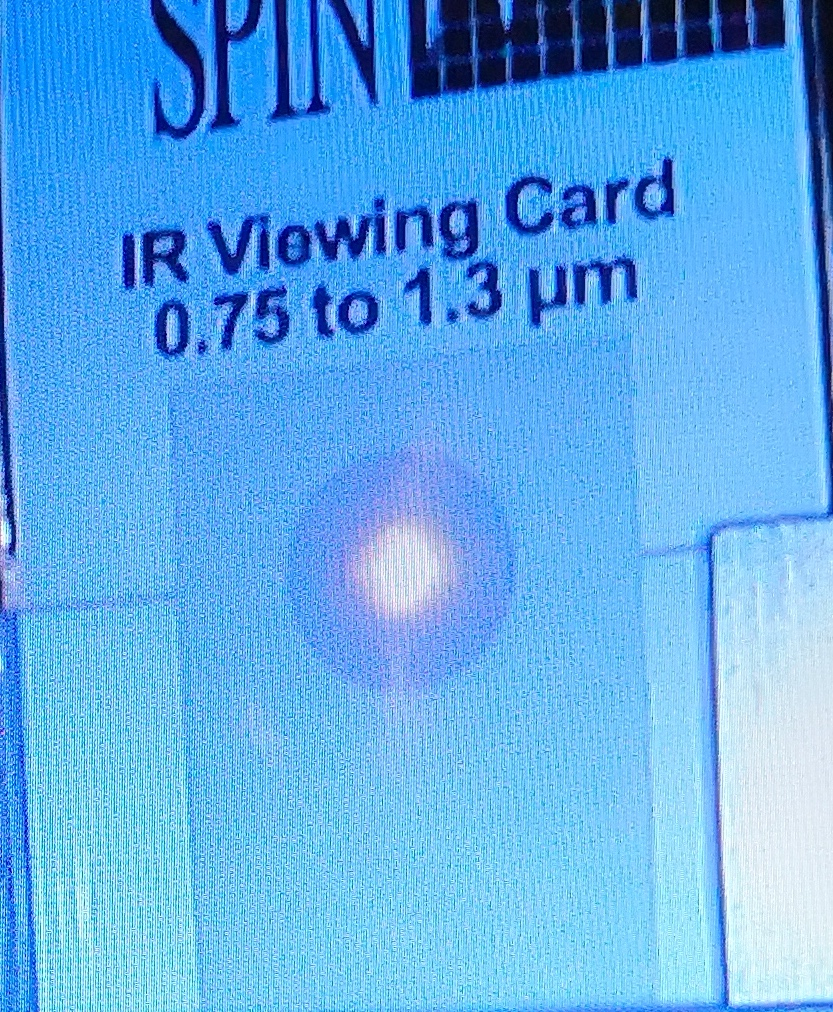
\includegraphics[width=\textwidth]{bilder/laser_before.jpg}
        \caption{Absorption and emission in the active medium are shown for a two state system. \cite{anleitungHeNe}}
        \label{fig:laser_before}
    \end{subfigure}
    \hfill
    \begin{subfigure}{0.49\textwidth}
        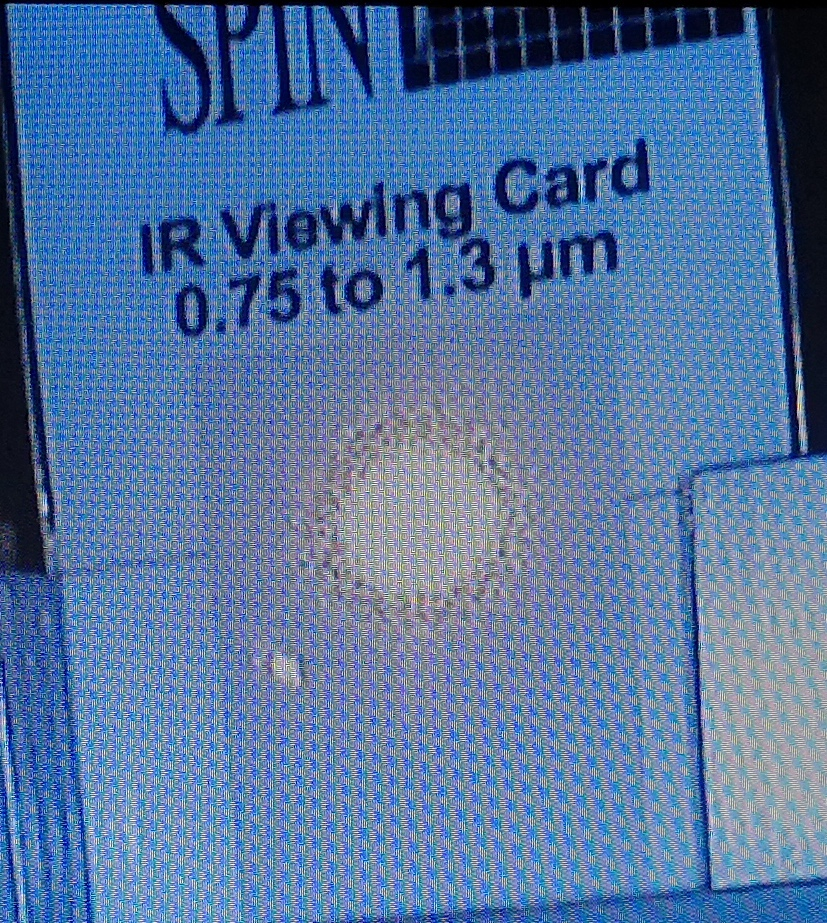
\includegraphics[width=\textwidth]{bilder/laser_after.jpg}
        \caption{Absorption and emission in the active medium are shown for a two state system. \cite{anleitungHeNe}}
        \label{fig:laser_after}
    \end{subfigure}
    \caption{images}
\end{figure}


\subsection{Rubidium fluorescence}
\begin{figure}[ht]
    \center
    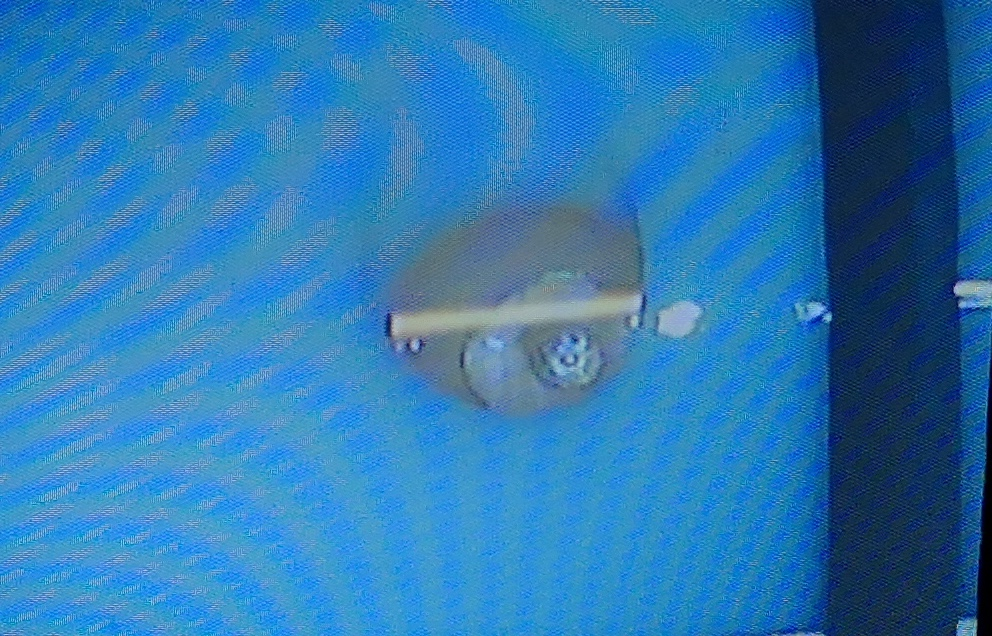
\includegraphics[width=0.8\textwidth]{bilder/fluorescence.jpg}
    \caption{Absorption and emission in the active medium are shown for a two state system. \cite{anleitungHeNe}}
    \label{fig:fluorescence}
\end{figure}


\subsection{Absorption spectrum of Rubidium}
\begin{figure}[ht]
    \center
    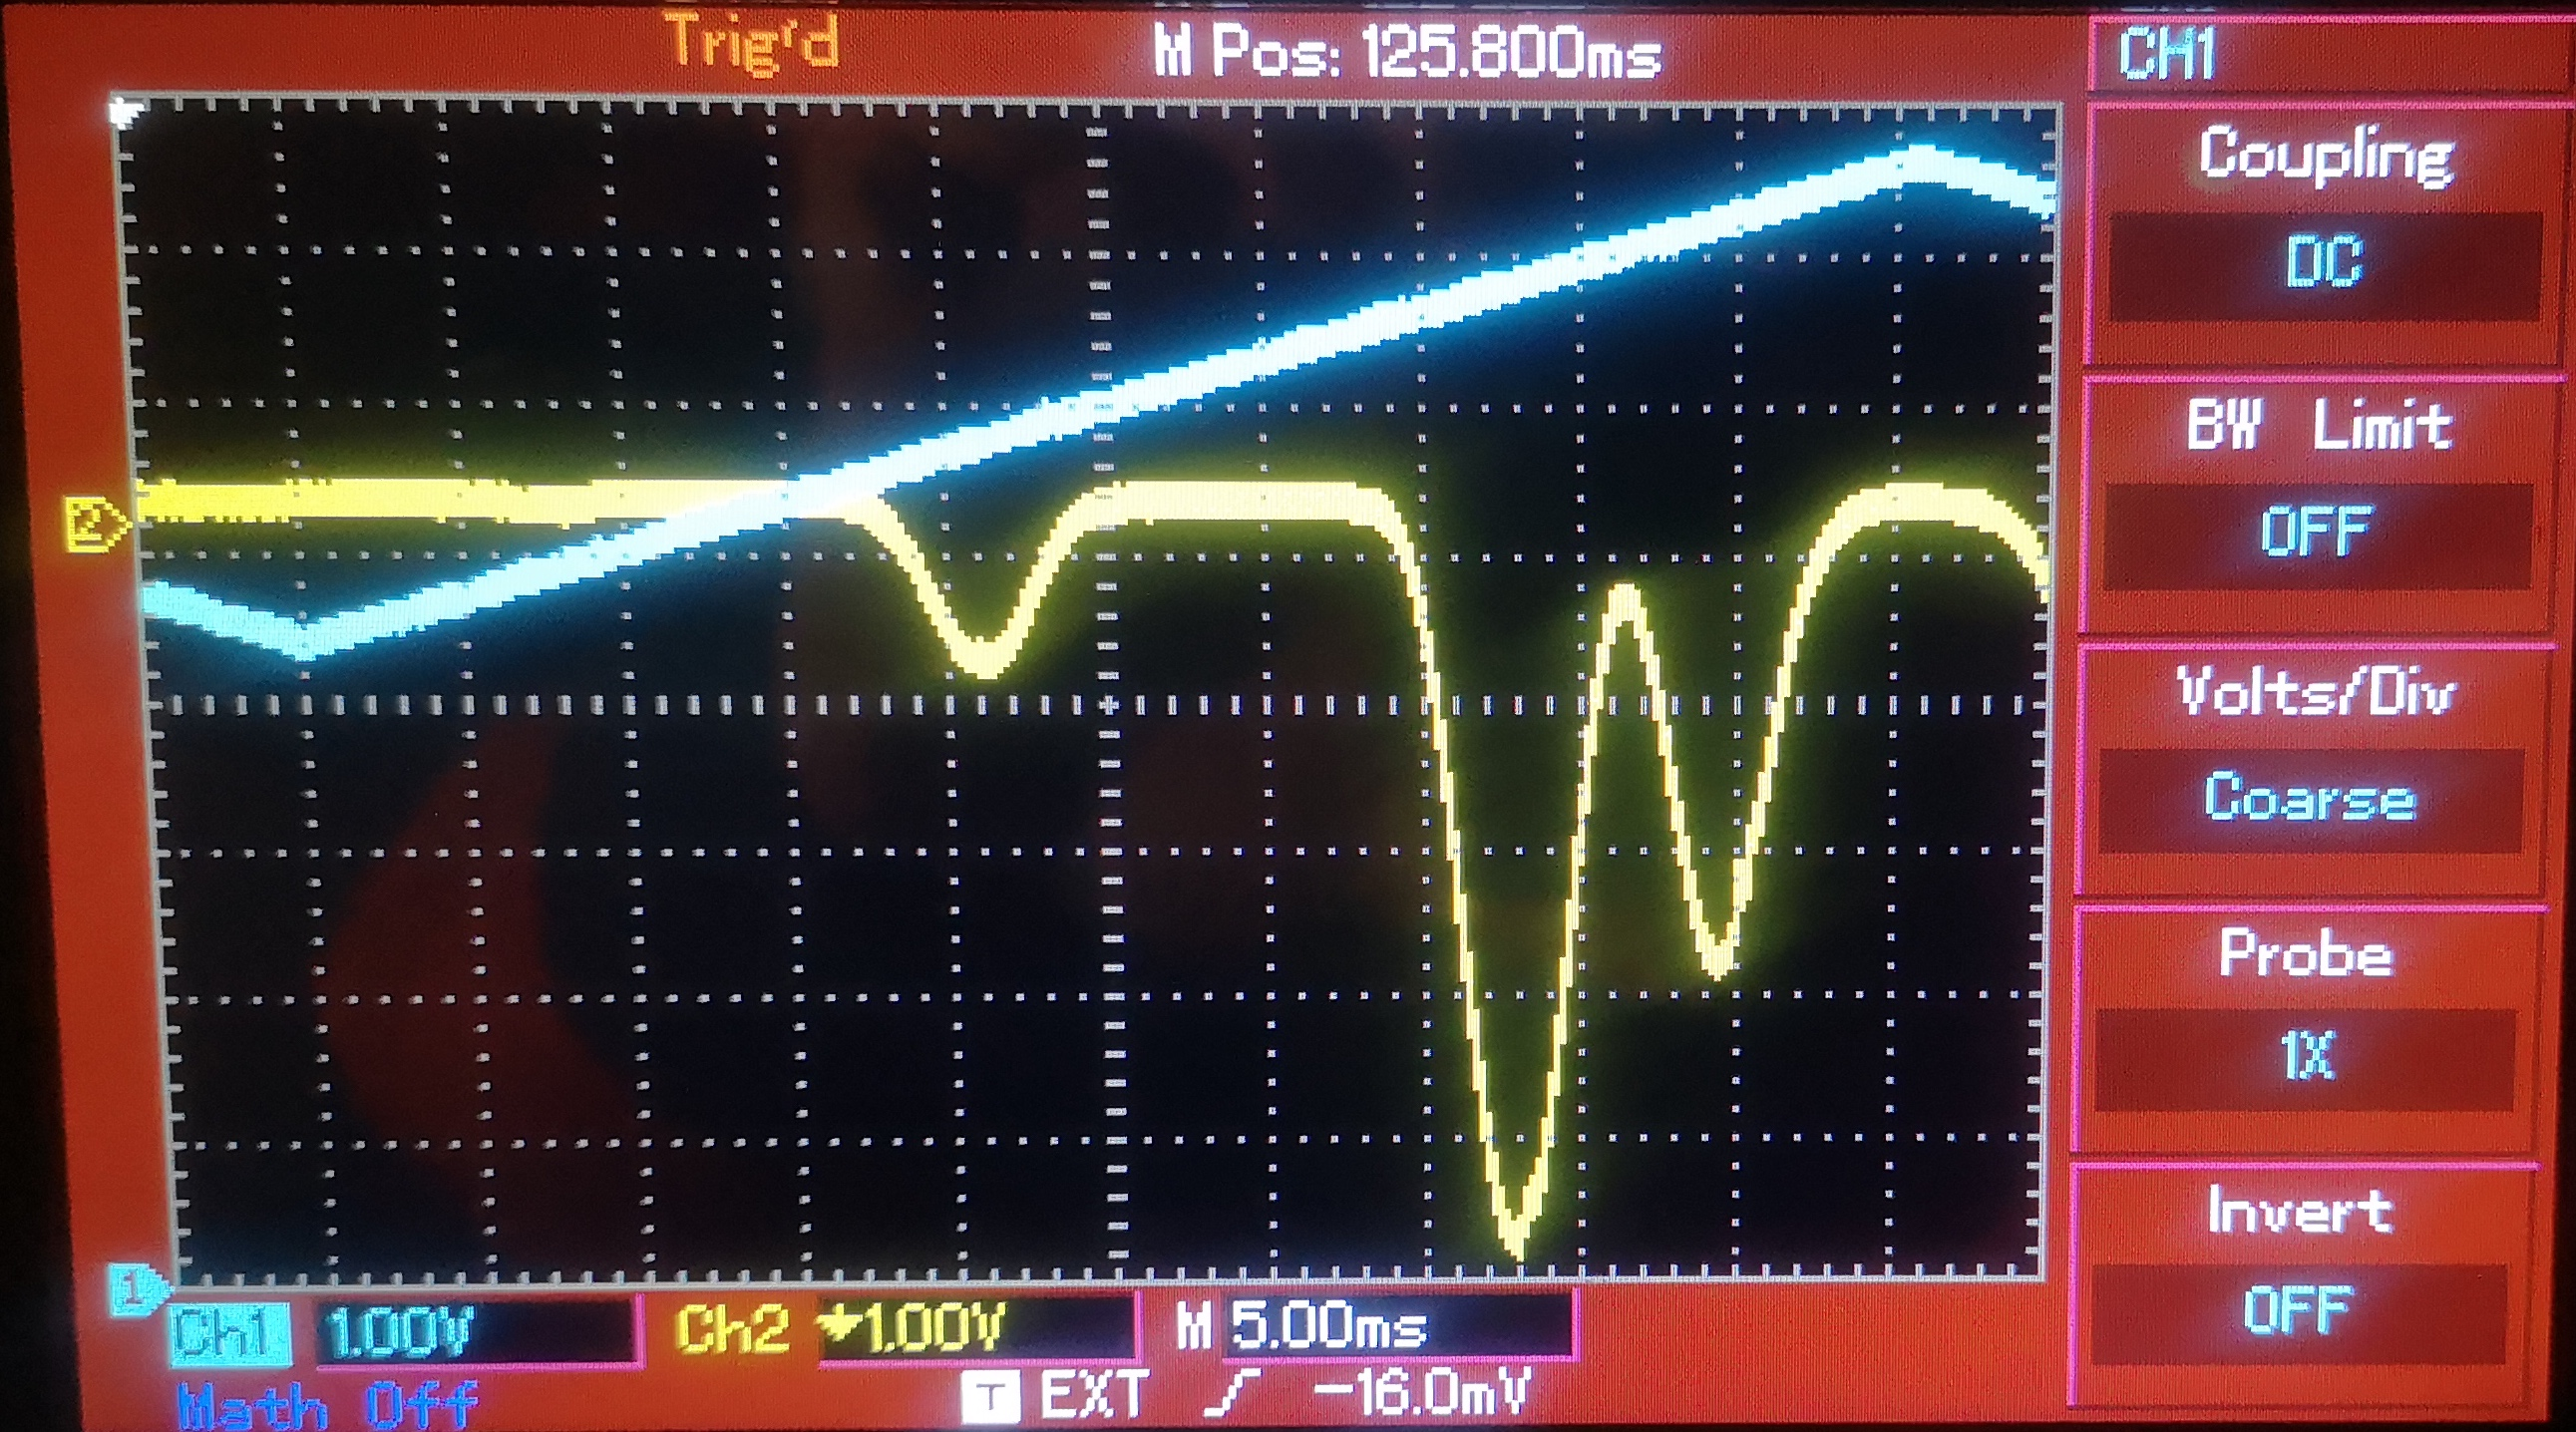
\includegraphics[width=0.8\textwidth]{bilder/spectrum.jpg}
    \caption{Absorption and emission in the active medium are shown for a two state system. \cite{anleitungHeNe}}
    \label{fig:spectrum}
\end{figure}